\chapter{Introducción al estudio del flujo de tráfico.}
\section{Introducción}
El flujo de tráfico es un fenómeno complejo. 

El movimiento de cada vehículo sobre la calzada puede analizarse tomando en consideración fenómenos físicos que permiten identificar su capacidad de aceleración, frenado o velocidad máxima, en función de sus características dinámicas y de la geometría de la carretera sobre la que circula.

Su comportamiento está altamnete condicionado por el comportamiento del conductor, el cual decide, en cada instante, las características de dicho movimiento, compatibles con los límites físicos.

Este hecho y la presencia simultánea sobre la carretera de otros conductores y vehículos, formando una ``corriente'' afectada, además, por diversos factores de la infraestructura y del medio, hace que el flujo de tráfico constituya un proceso entocástico, con variaciones aleatorias en vehículos y conductores (condiciones del medio: infraestructura, climatológicas, etc.).

La teoría de flujo de tráfico tiene por objeto la aplicación de leyes físicas, matemáticas y teorías de probabilidades para describir el comportamiento del tráfico / movimiento de los vehículos (``semilibres'') mediante estadística matemática.

Aplicaciones:
\begin{itemize}
    \item Estimación de la capacidad de vías.
    \item Determinación de retrasos probables en intersecciones.
    \item Análisis del impacto de sistemas mejorados de control de los vehículos sobre el flujo de tráfico
    \item Formación de colas.
\end{itemize}

\section{Modelos de tráfico}

Orientados a establecer relaciones entre variables asociadas al tráfico, tales como:
\begin{itemize}
    \item Valocidad
    \item Intensidad
    \item Densidad
    \item Evolución en el Tiempo (en algunos casos)
\end{itemize}

Pueden clasificarse en:
\begin{itemize}
    \item Modelos Microscópicos. Describen el movimiento de vehículos, considerados individualmente, y su interacción con los otros.
    \item Modelos Macroscópicos. Describen las relaciones entre velocidad, intensidad, y densidad en el flujo de vehículos.
\end{itemize}

En cierta forma, los fenómenos macroscópicos resultan de la agrupación de fenómenos microscópicos aunque no siempre posible formular las relaciones entre ellos a través de la adecuada formulación matemática.

\section{Variables básicas de tráfico}
No son variables independientes entre sí. Interesan las relaciones entre ellas que será objeto de estudio.
\begin{itemize}
    \item Intensidad
    \item Velocidad
    \item Sepatación Espacial
    \item Separación Temporales
    \item Densidad
\end{itemize}

\subsection{Intensidad de tráfico ($i$).}
Número de vehículos que pasan por una sección transversal de la carretera en una unidad de tiempo.

\subsubsection{Para tráfico ligero, ($\leq$ 200 VEH.HORA.CARRIL)}

Distribución de Poisson:
\begin{equation}
    P(i) = e^{q \cdot t} \frac{(q \cdot t)^i}{i!};\  i = 0,1,2...
\end{equation}

Donde:
\begin{itemize}
    \item $P(i)$: Probabilidad de que $i$ vehículos lleguen a una sección transversal fija de la carretera en un tiempo $t$ constante.
    \item $q$: Número medio de llegadas.
\end{itemize}

\begin{equation}
    \mu = \sigma^2 = q \cdot t
\end{equation}

\begin{equation}
    \gamma = \frac{\mu}{\sigma^2} = 1
\end{equation}

Donde:
\begin{itemize}
    \item $\mu$: Media o Esperanza
    \item $\sigma^2$: Varianza
    \item $\gamma$: Coef. Variación
\end{itemize}

\subsubsection{Distribución binomial, ($>$ 200 VEH./HORA.CARRIL)}

\begin{equation}
    P(i) = \binom{m}{i} \cdot p^i \cdot (1 - p)^{m-i}; i = 0,1,2,...m
\end{equation}

\begin{equation}
    \sigma^2 = m \cdot p \cdot q
\end{equation}

\begin{equation}
    \gamma = \frac{\mu}{\sigma^2} = \frac{m \cdot p}{m \cdot p \cdot q} = (1 - p)^{-1} \geq 1
\end{equation}

\subsubsection{Distribución binomial negativa, para representar régimenes sujetos a fuertes variacions}

\begin{equation}
    P(i) = \binom{i + K - 1}{i} \cdot p^K \cdot (1 - p)^i; i = 0,1,2... 
\end{equation}

\begin{equation}
    \mu = K \cdot (1 - p)/p
\end{equation}

\begin{equation}
    \sigma^2 = K \cdot (1 - p)/p^2
\end{equation}

\begin{equation}
    \gamma = p^2 / p < 1
\end{equation}


\subsection{Densidad de Tráfico ($K$)}
Número de vehículos por unidad de longitud que ocupan un tramo de carretera en un moemnto dado.

Colapso circulatorio:
\begin{itemize}
    \item Densidad máxima 160 vehículos por km
    \item Para velocidades moderadas $\approx$ 40 vehículos por km
\end{itemize}

\subsection{Velocidad($V$)}
\begin{itemize}
    \item Velocidad media de recorrido
    \item Velocidad media temporal o local: valor medio de las velocidades de los vehículos que pasan por una sección transversal de la carretera, durante un intervalo de tiempo.
    \item Velocidad media espacial: valor medio de las velocidades de todos los vehículos que, en un instante determinado, ocupan un tramo concreto de la carretera
\end{itemize}

Distribución normal:
\begin{equation}
    f(V) = \frac{1}{\sigma \cdot \sqrt{2 \cdot \pi}} e^{- (V - \mu)^2/2\cdot \sigma^2}
\end{equation}

Cuando la velocidad no preseneta una distribució aproximadamente simétrica se aplica una distribución tipo pearson (chi cuadrado o ji cuadrado).

\subsection{Intervalo ($h$)}
Tiempo transcurrido entre el paso de las partes himogéneas de dos vehículos consecutivos por una sección transversal de la carretera.
\begin{itemize}
    \item En tráficos débiles: distribuciones exponenciales negativas
    \item Al aumentar el tráfico: distribuciones mixtas
\end{itemize}

\subsection{Espaciamiento ($S$)}
Intervalo espacial entre dos secciones homogéneas de vehículos consecutivos.
\begin{itemize}
    \item Valor inverso de la densidad
\end{itemize}

\begin{equation}
    S = 1 / K
\end{equation}

\section{Modelos de flujo ininterrumpido de tráfico}

\begin{equation}
    i = V \cdot K
\end{equation}

Donde:
\begin{itemize}
    \item $i$: Intensidad (veh./hora)
    \item $V$: Velocidad (Km./h.)
    \item $K$: Densidad (Veh./km)
\end{itemize}

Todas las variables expresadas por sus valores medios.

Se han establecido modelos basados en observaciones del tráfico, que relacionan las anteriores variables dos a dos:
\begin{itemize}
    \item Relaciones velocidad-densidad-intensidad, considerando el modelo lineal entre v y k.
    \item Relaciones intensidad-densidad
    \item Relaciones velocidad-densidad-intensidad, considerando un modelo logarístmico entre v y k.
\end{itemize}

\paragraph{Modelo Lineal - Greenshield (1935)}
\begin{equation}
    V = V_L \cdot 1 - ( \frac{K}{K_C} )
\end{equation}

\paragraph{Modelo Logarítmico - Greenberg (1959)}
\begin{equation}
    V = V_m \cdot Ln ( \frac{K_c}{K} )
\end{equation}

$V_m$: Velocidad a la que la intensidad es máxima

\paragraph{Modelo Generalizados - Drew (1965)}
\begin{equation}
    V = V_L \cdot [1 - (\frac{K}{K_C})^\frac{n + 1}{2}]
\end{equation}

$n > -1$ y es lineal si $n = 1$

\section{Ondas de choque en el flujo de tráfico}

\begin{figure}[H]
    \centering
    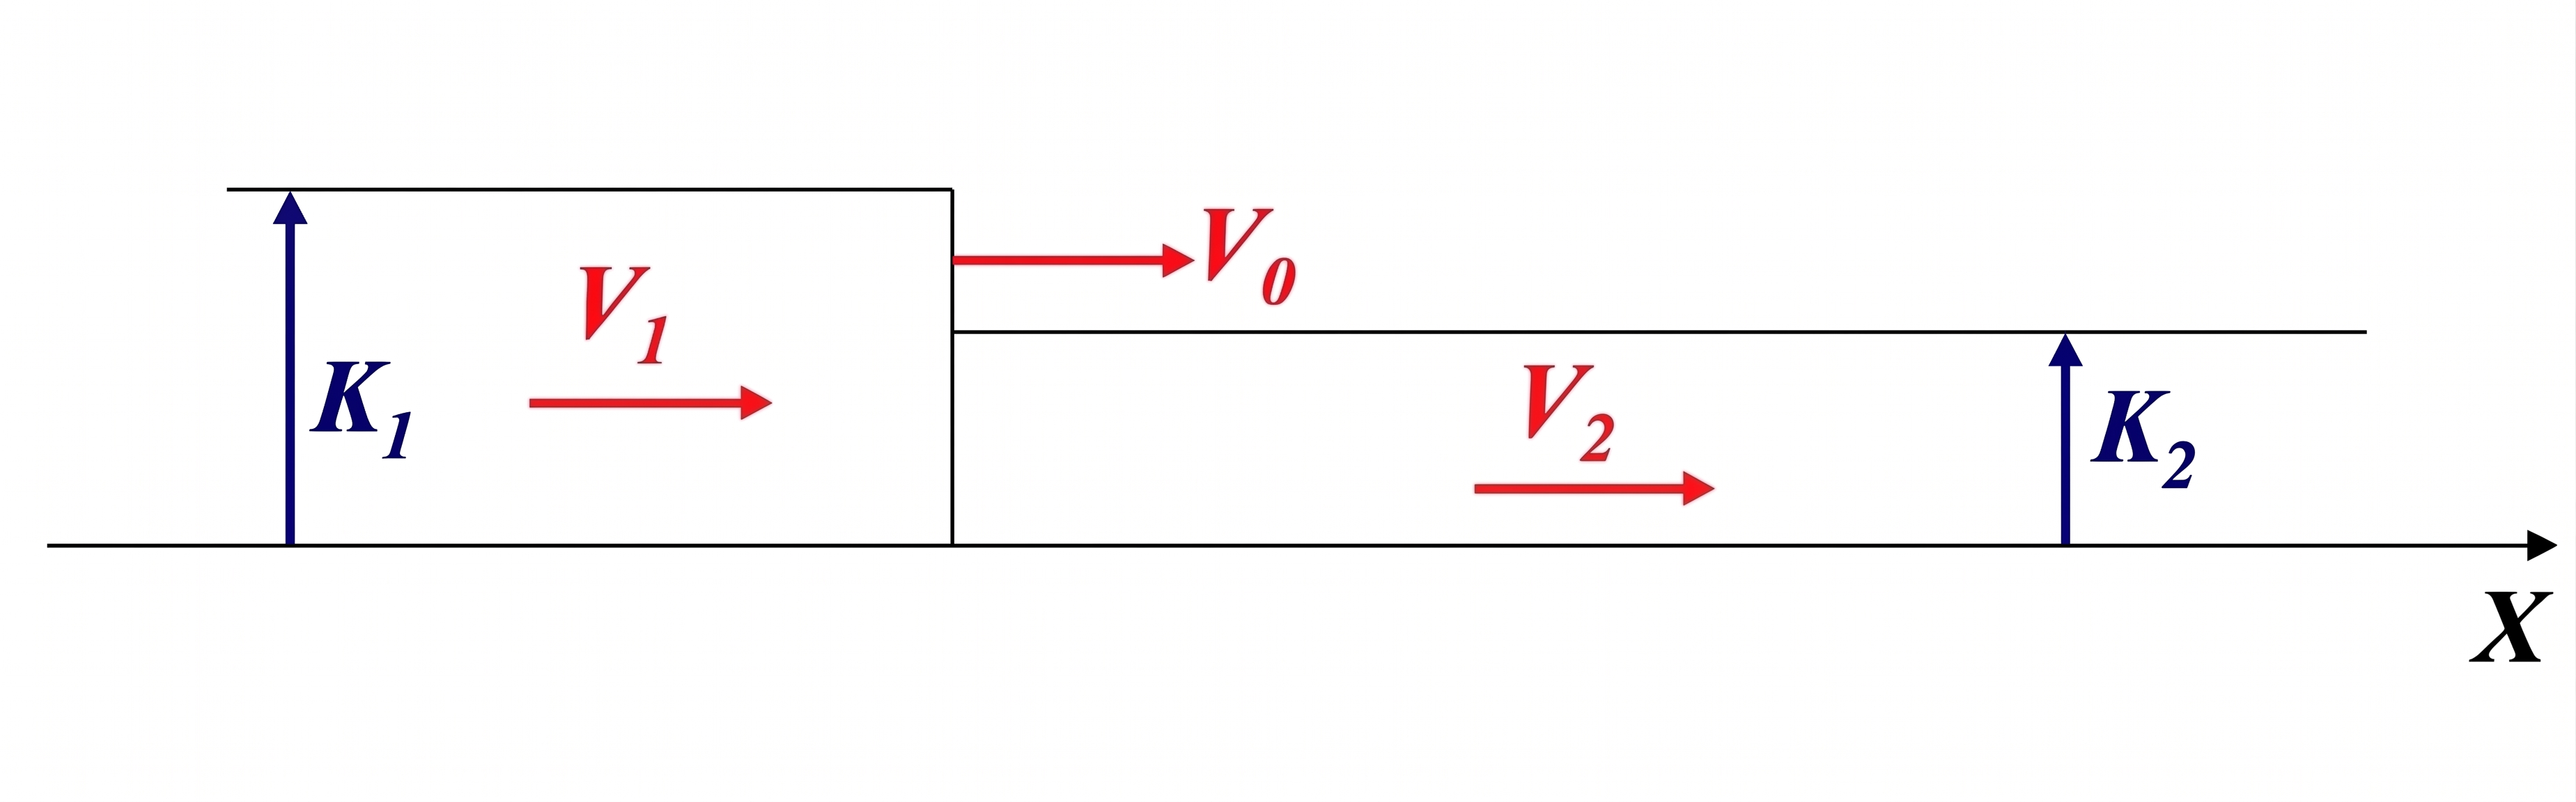
\includegraphics[width = \columnwidth]{Imagenes/Diagrama para el analisis de ondas de choque.png}
    \caption{Diagrama para el análisis de ondas de choque}
\end{figure}

``Movimiento de propagación de un cambio de densidad de flujo''

\section{Modelo de seguimiento de vehículos}

\section{Modelo para el cálculo de distancias mínimas de seguridad y capacidad de vías en autopistas automatizada}

\section{Capacidad y niveles de servicio en autopistas, autovías y carreteras convencionales}

\section{Análisis de colas de espera}